\chapter{Testautomatisierung}
\label{testautomatisierung}

Nach der Einführung der Methode im vorherigen Kapitel soll nun der entwickelte Prototyp erklärt werden.
Der entwickelte Prototyp lässt sich im \href{https://github.com/gernhard1337/graphql-primepath-tester}{GitHub} und im \href{https://git.informatik.tu-cottbus.de/sst/abschlussarbeiten/master/lorenz_tom/graphql-tester-prototyp}{BTU-GitLab} finden und testen.
Eine Anleitung findet sich in der Readme im Root-Verzeichnis.
Vorraussetzungen zum Ausführen der Anwendung ist Python und einige Dritt-Bibliotheken die in der Readme vermerkt sind.

\section{Auswahl der Bibliotheken}

Um die vorgestellte Methode umzusetzen war insbesondere wichtig, dass eine einfache und mächtige Bibliothek für die Definition und Bearbeitung von Graphen zur Verfügung steht.
Die erste Wahl fiel hierbei auf NetworkX, eine Graphenbibliothek für Python.
Sie wurde ausgewählt da schon einige Erfahrungen mit dieser Bibliothek exisitieren und somit eine effiziente Umsetzung ohne langwierige Einarbeitung möglich war.
Durch die Auswahl der Bilbiothek wurde gleichzeitig auch die Sprache Python festgelegt.
Einige weitere Bibliotheken wurden benötigt um den Applikationsstack zu vervollständigen.
Insgesamt waren Bibliotheken in den Bereichen Graphen, API-Kommunikation, JSON-Bearbeitung und Argumentgenerierung nötig um einen Prototypen umzusetzen.
Es werden nicht alle Bibliotheken eine Berücksichtigung hier finden, sondern nur diese, die einen signifikanten Einfluss auf das Programm haben und besonders herausstechen.

\subsection{NetworkX}

NetworkX ist eine Python-Biblitohek für \textit{Erstellung, Manipulation und Untersuchung der Struktur, Dynamik und Funktionen komplexer Netzwerke}~\cite[vgl. Startseite]{networkx}
Mit einer Star-Anzahl von \textit{12.8k}\cite{networkxgithub} auf GitHub ist networkX eine sehr beliebte Bibliothek.
NetworkX ist die ideale Wahl um Graphen zu erstellen für unseren Use-Case denn es nimmt jeden möglichen Datentypen als Wert für einen Knoten und Kante.
Wir können also sehr simpel Graphen definieren.
Für ein enfaches Beispiel von Author, Book, Publisher und deren Verbindungen benötigen wir nur folgende Zeilen Code:

\begin{lstlisting}[language=Python]
import networkx as nx

G = nx.Graph()
G.add_edge("Query", "Book", "book")
G.add_edge("Query", "Author", "author")
G.add_edge("Query", "Publisher", "publisher")

G.add_edge("Publisher", "Book", "book")
G.add_edge("Book", "Publisher", "publisher")

G.add_edge("Book", "Author", "author")
G.add_edge("Author", "Book", "book")
\end{lstlisting}

Diese wenigen Zeilen reichen aus um unseren Graphen mit allen Knoten und Kanten zu definieren.
Wir können hier auch direkt das Kantengewicht mit dem Feldbezeichner angeben, so ist es möglich, dass wir sofort
wissen, welche Kante genutzt werden muss um zum nächsten Typ zu gelangen.
Auf diesem Graphen können wir dann diverse Algorithmen ablaufen lassen.
Diverse Hilfsfunktionen helfen dabei eine effiziente Programmierung zu erlangen.
Hierbei seien insbesondere folgende Hilfsfunktionen genannt:

\subsubsection{draw}
    \begin{lstlisting}[language=Python]
nx.draw(G, with_labels=True)
    \end{lstlisting}

Zeichnet einem den erstellten Graphen in ein beliebiges Format.
So fällt es einfach große Graphen darzustellen.

\subsubsection{shortest\_path}
    \begin{lstlisting}[language=Python]
shortest_path = nx.shortest_path(G, Node1, Node5)
    \end{lstlisting}

Die Funktion $shortest\_path$ gibt eine Liste von Kanten zurück, die den kürzesten Weg zwischen zwei
Knoten angibt.

\subsubsection{neighbors}
    \begin{lstlisting}[language=Python]
G.neighbors(Node)
    \end{lstlisting}
Diese Funktion liefert alle Nachbarn eines Knotens.

\subsubsection{simple\_paths}

Diese Funktion liefert uns alle einfachen Pfade wie in Kapitel~\ref{testpfade} gewünscht.
So ist es uns direkt möglich, aus dem Ergebnis dieser Funktion die PrimePfade herauszufiltern.
Somit erleichtert die Biblitohek uns die Berechnung der Pfade stark.

\begin{lstlisting}[language=Python]
nx.all_simple_paths(G, source=start_node, target=end_node)
\end{lstlisting}


\subsection{Faker}
Die gewählte Argumentgenerierungsbibliothek ist \textit{Faker}\cite{fakergithub}.
Mit \textit{16k}\cite{fakergithub} Sternen auf GitHub ist Faker auch eine beliebte Bilbiothek.
Faker ist eine Bilbiothek die es sehr einfach macht Daten zu generieren.
Da wir im Kontext von GraphQL Argumenten nur sehr einfache Datentypen als Argumente benötigen reicht uns diese
Bibliothek komplett aus da sie es schafft uns schnell und unkompliziert Daten in genau dem Format zu generieren wie wir sie brauchen.
Angenommen wir benötigen einen String der 10 Zeichen lang ist, so reicht eine Zeile:

\begin{lstlisting}[language=Python]
random_string = fake.pystr(min_chars=10, max_chars=10)
\end{lstlisting}

Selbiges falls wir eine Zufallszahl benötigen zwischen 1 bis 1000

\begin{lstlisting}[language=Python]
random_number = fake.random_int(min=1, max=1000)
\end{lstlisting}

Dieses Schema des Einzeilers gilt für alle simplen $SCALAR$ Types in GraphQL.
Daher fällt die Wahl für die Datengenerierung auf diese Bibliothek.

\subsection{PyTest}

Um die gewünschte Reproduzierbarkeit aus Kapitel~\ref{testf} zu erreichen, nutzen wir das Testframework PyTest.
Dies ist ein Testframework für Python welches eine simple und einfache Testdefinition ermöglicht.
Ein Test für eine einfache Funktion $inc$ kann mit $test\_inc$ umgesetzt werden.

\begin{lstlisting}[language=Python]
def inc(x):
    return x + 1

def test_inc():
    assert inc(3) == 5
\end{lstlisting}

Die einfache Syntax von PyTest reicht für unseren Anwendungsfall vollkommen aus.
Gleichzeitig sind Imports in PyTest sehr einfach umzusetzen daher nutzen wir dieses Testframework.
\newpage

\section{Umsetzung der Methode}

Für die Umsetzung der Methode werden wir durch die einzelnen Teile des Codes gehen und die jeweiligen Schritte erklären.
Hierbei gehen wir chronologisch in den einzelnen Schritten vor so wie in der Methode definiert.
Im Allgemeinen funktioniert der Prototyp so wie in dem Sequenzdiagramm in Abbildung~\ref{sqzd} gezeigt.

\begin{figure}[H]
    \begin{center}
        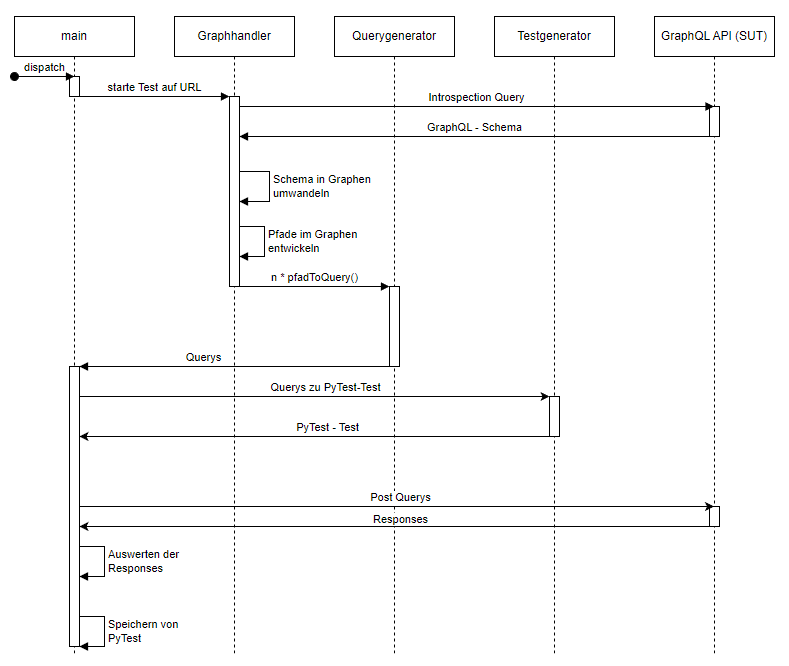
\includegraphics[width=\textwidth,height=\textheight,keepaspectratio]{img/sequenz}
    \end{center}
    \caption{Sequenzdiagramm des Prototypens}
    \label{sqzd}
\end{figure}

Hierbei sind auch die einzelnen Module zu erkennen.
Dabei sind die Module main, Graphhandler, Querygenerator und Testgenerator Teile des Prototypens.
Das Modul GraphQL API stellt das zu testende System dar und ist extern.

\subsection{Schema in Graph abbilden}

Wie in der Vorstellung der Methode in Kapitel~\ref{schemagraph} bilden wir das GraphQL-Schema in einem NetworkX-Graphen ab.
Um die Informationen zu erlangen die für die Bildung des Graphens wichtig sind führen wir zuerst die Introspection-Query~\ref{introspection-query} aus.
Das Ergebnis ist dann das vollständige GraphQL-Schema der API.
Hierbei sei angemerkt, dass einige GraphQL APIs so eine Introspection-Query verbieten, sei es einerseits durch direktes verbieten oder ein Tiefenlimit in den Querys.
Egal was hierbei der Fall ist, die zu testende API muss unsere Introspection-Query~\ref{introspection-query} unterstützen, da wir sonst keine Informationen erlangen können.
Die Query wird mit einem simplen HTTP-POST an die zu testende URL gesendet.

\begin{lstlisting}[language=Python]
r = requests.post(testUrl, json={'query': queries.introspection_query})
json_data = json.loads(r.text)
\end{lstlisting}

Und die Response wird als JSON-Objekt in $json\_data$ gespeichert.
Es wurde ein Modul $Graphhandler$ entwickelt, dass verschiedene Graphoperationen Übernimmt.
Im Graphhandler ist eine Funktion $buildGraph$ definiert.
Diese generiert einen Graphen von einem gegebenen Startknoten, einem leeren Graphen und dem Schema.
Hierbei werden nur erreichbare Knoten vom Startknoten berücksichtigt.
Setzt man den Startknoten auf den Knoten $Query$ so inkludieren wir auf diese Weise nur alle erreichbaren Teile des Graphens ausgehend von $Query$.
Dies ist insofern sinnvoll da andere Typen, wenn sie nicht von $Query$ aus erreichbar sind, nicht Teil des Testraumes wären da diese in keiner validen Anfrage vorkommen können.
Die Funktion, die den Graphen generiert ist in Abbildung~\ref{graphbuild} dargestellt.

\begin{figure}
    \begin{lstlisting}[language=Python]
def buildGraph(graph, type_name, type_dict):
    if type_name.startswith(nonSchemaTypePrefix) or type_name in baseDatatypes:
        pass
    else:
        for adjacentNode in type_dict[type_name]['fields']:
            if graph.has_edge(type_name, adjacentNode['type']['name']):
                return
            else:
                if adjacentNode['type']['name'] and adjacentNode['type']['name'] not in baseDatatypes:
                    graph.add_edge(type_name, adjacentNode['type']['name'])
                    graph[type_name][adjacentNode['type']['name']]["data"] = adjacentNode
                    buildGraph(graph, adjacentNode['type']['name'], type_dict)
                if adjacentNode['type']['kind'] == 'LIST' and adjacentNode['type']['ofType']['name'] not in baseDatatypes:
                    graph.add_edge(type_name, adjacentNode['type']['ofType']['name'])
                    graph[type_name][adjacentNode['type']['ofType']['name']]["data"] = adjacentNode
                    buildGraph(graph, adjacentNode['type']['ofType']['name'], type_dict)
    \end{lstlisting}
    \caption{Funktion die einen Graphen aufspannt}
    \label{graphbuild}
\end{figure}

Die Funktion buildGraph arbeitet rekursiv.
Vom Startknoten (im Allgemeinen $Query$) aus rufen wir die Funktion auf allen Folgeknoten von Query auf.
Dies sind alle Knoten die den Type $OBJECT$ besitzen und nicht mit einem $\_\_$ beginnen oder ein Basisdatentyp sind.
GraphQL kann eigene Objekte definieren welche mit $\_\_$ starten, diese schließen wir explizit aus genau wie alle $SCALAR$ Types.
Jeder Knoten definiert nun in seinem $fields$ Eintrag zu welchen Feldern er Beziehungen hat.
Hierbei muss unterschieden werden, dass ein Eintrag entweder vom Type $OBJECT$ oder $LIST$ sein kann, um zulässig zu sein.
Sollte es sich um einen $LIST$ Eintrag handeln müssen wir prüfen, von welchem Type die $LIST$ ist.
Wenn ein Knoten nun unsere Bedingungen erfüllt, so wird dieser dem Graphen hinzugefügt und auf ihm selbst wird $buildGraph$ ausgeführt.
So erlangen wir die gesamte Graphstruktur da ausgehend von Query jeder erreichbare Knoten hinzugefügt wird und dann von diesem Knoten eben wieder alle erreichbaren Knoten
hinzugefügt werden.
\newpage
\subsection{Pfade aus Graph bilden}

Der Graphhandler implementiert verschiedene Abdeckungskriterien.
Das Tool benötigt im späteren Verlauf lediglich eine Liste $paths$ aller Pfade, die für die Testgenerierung berücksichtigt werden sollen.

\begin{figure}[H]
    \begin{lstlisting}[language=Python]
paths = graphhandler.generate_prime_paths("Query", graph)
    \end{lstlisting}
    \caption{$paths$ als Liste von Pfaden für ein Abdeckungskriterium}
\end{figure}

Da wir jedoch in Kapitel~\ref{fazitcov} feststellten, dass die PrimePfade-Abdeckung am geeignetsten ist, erklären wir dieses Kriterium hier.
Die PrimePfad Abdeckung ist durch die Funktion $generate_prime_paths$ implementiert.
Diese Funktion verknüft dabei allerdings nur zwei andere Funktionen.

\begin{figure}[H]
    \begin{lstlisting}[language=Python]
def generate_prime_paths(startknoten, g):
    return shortest_path_to_prime(g, startknoten, get_prime_paths(g, startknoten))
    \end{lstlisting}
    \caption{valide PrimePfad Generierung}
\end{figure}

Da PrimePfade nicht im Query Knoten starten müssen, rufen wir zuerst die Funktion $get\_prime\_paths$ auf um eine Liste
aller PrimePfade zu bekommen.
Da jedoch ein Pfad stets im Query-Knoten starten muss, rufen wir anschließend $shortest\_path\_to\_prime$.
Diese Funktion ermittelt den kürzesten Weg vom QueryKnoten zum Startknoten des PrimePfades.
So können wir sicherstellen, dass die generierten Pfade stets valide Testpfade sind und dennoch alle PrimePfade abdecken.
Die Funktion $get\_prime\_paths$ ist in Abbildung~\ref{getprime} dargestellt.

\begin{figure}
    \begin{lstlisting}[language=Python]
def get_prime_paths(G, start_node):
    all_prime_paths = []
    nodes = list(G.nodes())

    for end_node in nodes:
        if end_node == start_node:
            continue
        simple_paths = list(nx.all_simple_paths(G, source=start_node, target=end_node))

        # Ein Pfad ist prime, wenn er kein Teilpfad ist
        prime_paths_for_end_node = []
        for path in simple_paths:
            is_prime = True
            for other_path in simple_paths:
                if set(path).issubset(set(other_path)) and path != other_path:
                    is_prime = False
                    break
            if is_prime:
                prime_paths_for_end_node.append(path)

        all_prime_paths.extend(prime_paths_for_end_node)
    return all_prime_paths
    \end{lstlisting}
    \caption{PrimePfad Generierung}
    \label{getprime}
\end{figure}

Sie nutzt die Gegebenheit, dass Anfragen zwar im Query-Knoten starten müssen, jedoch jeder andere Knoten des Graphens ein potentieller Endknoten ist.
Jeder Knoten wird dabei einmal als Endknoten behandelt und die einfachen Pfade von Query-Knoten zu diesem Knoten werden ermittelt.
Anschließend werden die Pfade so gefiltert, dass nur die längsten Pfade, die keine Unterpfade haben zurückgegeben werden.
Dies entsprich laut Definition~\ref{primepfad} einem PrimePfad und der Algorithmus ist Deckungsgleich mit~\cite[Finding Prime Test Paths S.39]{software-testing}.

\newpage
\subsection{Querys aus Pfad ermitteln}

Die entwickelten Pfade werden in diesem Schritt nun in Querys umgewandelt, sodass diese an die GraphQL-API
gestellt werden können.
Eine Query beginnt in GraphQL immer im Query-Knoten und so beginnen auch alle unseren ermittelten Pfade in diesem Knoten.
Da wir die Wahrscheinlichkeit erhöhen wollen, dass ein Pfad gut abgedeckt wird, generieren wir pro Pfad nicht einen Test sondern führen eine
Variable $testPerPath$ ein, die festlegt, wieviele Querys pro Pfad generiert werden sollen.
Standardmäßig legen wir fest: $testPerPath = 5$.
Um Querys aus einem Pfad zu erstellen wurde der $querygenerator$ entwickelt.
Der Querygenerator hat die Methode $pathToQuery$ welche den Pfad, ein Typedict und den Graphen erwartet.
Das Typedict ist ein Python-Dict, dass alle Informationen über das Schema enthält.
Die Funktion erstellt nun eine Query indem der angegebene Pfad abgelaufen wird.
Diese Funktionalität setzt die rekursive Funktion $resolvePathTillOnlyScalarTypesOrEnd(path, typedict, graph, query="")$ um die in Abbildung~\ref{respath} dargestellt ist.

\begin{figure}
    \begin{lstlisting}[language=Python]
def resolvePathTillOnlyScalarTypesOrEnd(path, typedict, graph, query=""):
    if path:
        edge = path.pop(0)
    else:
        return query
    edge_data = graph[edge[0]][edge[1]]["data"]
    if len(edge_data['args']) < 1:
        if edge_data["type"]["kind"] == "SCALAR":
            query = query + " " + edge_data["name"] + " "
        else:
            query = query + " " + edge_data["name"] + " { " + addScalarTypes(edge_data["type"], typedict, edge_data["name"]) + " " + resolvePathTillOnlyScalarTypesOrEnd(path, typedict, graph, query) + " } "
    else:
        argString = edge_data['name'] + "("
        for args in edge_data['args']:
            argString = argString + args["name"] + ": " + resolveArg(args["type"], typedict) + ", "
        argString = argString + ")"
        query = query + argString + " { " + addScalarTypes(edge_data["type"], typedict, edge_data["name"]) + " " + resolvePathTillOnlyScalarTypesOrEnd(path, typedict, graph, query) + " } "
    return query
    \end{lstlisting}
    \caption{Pfadumwandlung in Query}
    \label{respath}
\end{figure}

Die Funktion arbeitet dabei so, dass sie für jeden Ausgangspunkt einer Kante alle $SCALAR$ Felder hinzufügt.
So wird sichergestellt, dass alle einfachen Felder eines Objektes abgefragt werden.
Es kann so validiert werden, dass das Objekt übereinstimmt mit der Schema-Definition.
Sind alle $SCALAR$ Types hinzugefügt, so wird geprüft, welches Feld vom Type $OBJECT$ hinzugefügt werden muss, um die Kante zum nächsten Knoten abzubilden.
Sollte diese Kante Einträge im $args$ Feld besitzen, so werden die Argumente generiert.
Da Argumente nur $SCALAR$ Types oder Aggregationen von $SCALAR$ Types sein können, benötigen wir Datengeneratoren für die Standarddatentypen.
Die Zuweisung der Datengeneratoren geschieht hierbei mit der Funktion $resolveArg$.
Benötigt ein $OBJECT$ Feld nun Argumente, so werden diese der Query hinzugefügt indem mit $resolveArg$ die Argumente zur Verfügung gestellt wurden.
Anschließen wird die Kante aus der Liste des Pfades entfernt und die Funktion wieder rekursiv aufgerufen.
Abbruchbedingung ist, dass der Pfad keine Kanten mehr besitzt.
Wenn der Pfad keine Kanten mehr besitzt, so ist die entwickelte Query ein Test, der den Pfad abdeckt.
Es sei angemerkt, dass durch die zufällige Argumentgenerierung keinesfalls garantiert ist, dass bei der Testausführung dann der volle Pfad getestet wird.
Sollte zum Beispiel ein Pfad direkt am Anfang Argumente benötigen, diese aber jedoch zu keinen Daten des SUT passen, so ist es sehr
wahrscheinlich, dass der Test erfolgreich sein wird, ohne dass der eben entwickelte Pfad wirklich komplett getestetet wird.
\newpage

\subsection{Tests ausführen \& Testdatei generieren}

Bevor wir die Tests ausführen, werden diese im PyTest-Format gespeichert.
Hierzu wird eine Datei angelegt, die alle nötigen Imports enthält.
Anschließend wird für jede Query ein eigener Test angelegt und die Auswertung festgeschrieben.
Dafür existiert die Funktion $generateTestFromQuery$ im Modul Testgenerator.
Ein so erstellter PyTest ist in Abbildung~\ref{pytestt} dargestellt.

\begin{figure}[H]
    \begin{lstlisting}[language=Python]
def testQuery6aa8b26(caplog):
    caplog.set_level(logging.WARNING)
    response = requests.post(testUrl,json={'query':"{...}")
    response_as_dict = json.loads(response.text)
    measurement = queries.compareQueryResults(response_as_dict, "{...}")
    if measurement["expectedPathLength"] > measurement["pathLengthFromResult"]:
        logging.warning(" Test hat nicht 100% Abdeckung ")
    assert response.status_code == 200
    \end{lstlisting}
    \caption{PyTest einer Query}
    \label{pytestt}
\end{figure}

Nachdem mit den PyTests die Querys reproduzierbar gemacht wurden, führen und werten wir diese aus.
Hierbei nutzen wir den Code aus Abbildung~\ref{testt}.
Eine Query wird als HTTP-POST an das SUT gestellt, die Antwort wird dann auf ihre Pfadlängen hin untersucht und in
einer Datei abgespeichert.

\begin{figure}[H]
    \begin{lstlisting}[language=Python]
queryResults = []
for testQuery in primePathQueries:
    r = requests.post(testUrl, json={'query': testQuery}, headers=HEADERS)
    response_as_dict = json.loads(r.text)
    measurement = queries.compareQueryResults(response_as_dict, testQuery)
    queryResults.append([testQuery, r, measurement])
    f.write(" => ".join([testQuery, r.text]))
    f.write("\n")
f.close()
    \end{lstlisting}
    \caption{Ausführen einer Testquery}
    \label{testt}
\end{figure}

Um die Tests auszuführen, senden wir alle zuvor generierten Querys an das SUT.
Die Antworten werden zuerst gespeichert und dann später ausgewertet.

\subsection{Testauswertung}

Die Testauswertung erfolgt, wie zuvor gesehen, in zweierlei Arten.
Einerseits werden Tests ad-hoc ausgeführt.
Andererseits wird eine Datei mit PyTests generiert.
Die Auswertung der Testquerys in der PyTest Datei erfolgt nach PyTest Standard, dabei werden Hinweise geliefert falls etwas abweicht von der Erwartung.
Eine Auswertung der Testquerys die direkt ausgeführt wurden erfolgt nach einer Kategoriesierung.
Die Kategoriesierungen sind \textbf{Good\_Test},\textbf{Perfect\_Test},\textbf{malformed\_Test} und \textbf{confirmed\_failed\_Test}.
Ein \textbf{Good\_Test} ist ein Test, der keinen Fehler erzeugt hat allerdings ist die erwartete Pfadlänge von der Response nicht erfüllt worden, es war also ein Test
der nicht die komplett gewünschte Abdeckung erreicht hat.
\textbf{Perfect\_Test} sind Tests, die keinen Fehler erzeugt haben und die erwartete Pfadlänge entspricht der Pfadlänge der Response.
Eine solche Query hat den Pfad, der zu testen war, ideal abgedeckt.
\textbf{malformed\_Test} sind Tests, die fehlerhaft sind aber allerdings aufgrund von Generierungsfehler vom Prototypen.
\textbf{confirmed\_failed\_Test} sind Tests bei denen wir tatsächlich einen Fehler bekommen.
Die Fehlerhaften Tests werden dann im folgenden Ausgegeben mit der konkreten Fehlerbeschreibung, sodass eine Fehleranalyse möglich wird.
Um Maß darüber zu halten, wie viele Tests in welcher Kategorie sind wurde eine Auswertung geschrieben welche in Abbildung~\ref{auswert} gezeigt ist.

\begin{figure}
    \begin{lstlisting}[language=Python]
successfull = 0
perfect = 0
own_failure = 0
server_failures = 0
testCount = 0

for queryResult in queryResults:
    testCount = testCount + 1
    if any(substring in queryResult[1].text for substring in ["GRAPHQL_PARSE_FAILED", "GRAPHQL_VALIDATION_FAILED"]):
        own_failure = own_failure + 1
    elif "INTERNAL_SERVER_ERROR" in queryResult[1].text or r.StatusCode == 500:
        server_failures = server_failures + 1
    elif "data" in queryResult[1].text and queryResult[2]["expectedPathLength"] > queryResult[2]["pathLengthFromResult"]:
        successfull = successfull + 1
    elif "data" in queryResult[1].text and queryResult[2]["expectedPathLength"] == queryResult[2]["pathLengthFromResult"]:
        perfect = perfect + 1
    \end{lstlisting}
    \caption{Auswertung der Antworten}
    \label{auswert}
\end{figure}
\newpage

\section{Zusammenfassung der Implementation}

Der Python Prototyp stellt eine Implementierung der Methode aus Kapitel~\ref{testentwurf} dar.
Wie wir später sehen werden ist der Prototyp in der Lage reale Fehler in GraphQL-APIs zu finden.
Die modulare Aufbauweise des Prototypens erlaubt es, dass zukünftige Anpassungen an der Software einfach umsetzbar sind.
So sind die Module thematisch getrennt und das anpassen sowie auswechseln einzelner Module ist möglich ohne die Funktionsweise
der anderen zu beeinträchtigen.


